\documentclass[a4paper,12pt]{article}
\usepackage[utf8]{inputenc}
\usepackage[english]{babel}
\usepackage{amsmath,amssymb}
\usepackage{graphicx}
\usepackage{listings}
\usepackage{xcolor}
\usepackage{hyperref}
\usepackage{geometry}
\geometry{margin=2.5cm}

\title{Project Documentation \\ Decoder Implementation of the RISC-V Efficient Trace}
\author{Righi Samuele / UNIBO, Dipartimento di Informatica - Scienza e Ingegneria }
\date{July 1, 2025}

\begin{document}

\maketitle
\tableofcontents
\newpage


% -------------------------------
\section{System Overview}
The goal of this project \cite{trace_decoder} is to implement the \textit{Efficient Trace for RISC-V}\cite{riscv_trace_spec} specification. 

\begin{figure}[h]
    \centering
    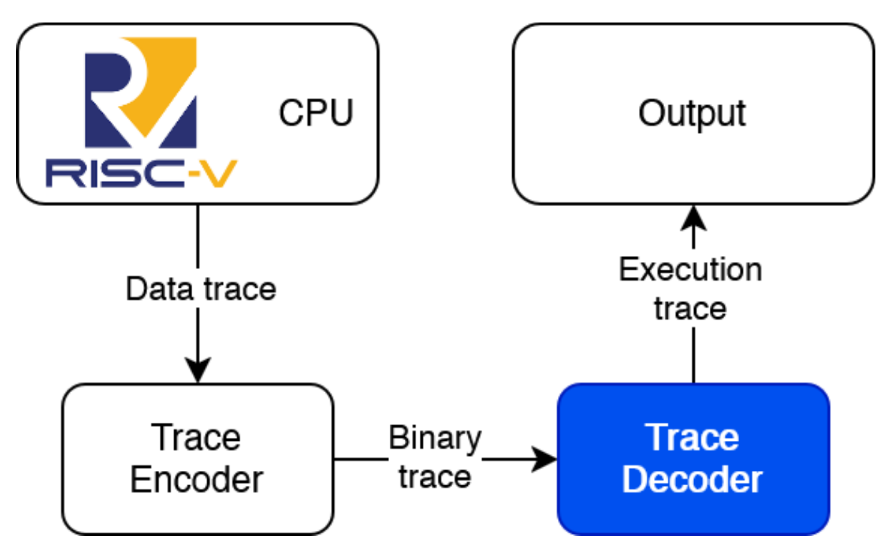
\includegraphics[width=0.6\linewidth]{img/tracing_diagram.png}
\end{figure}


More specifically, it focuses on developing a trace decoder that converts the binary trace data generated and published by the encoder into structured packets. These packets are then used to reconstruct the program’s execution trace at the assembly level.

\begin{figure}[h]
    \centering
    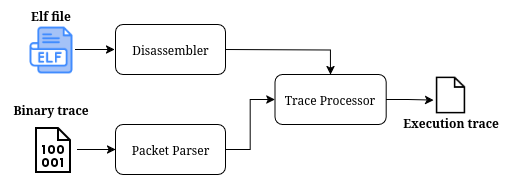
\includegraphics[width=0.8\linewidth]{img/trace_processing_flow.png}
\end{figure}

Main components of the system include:
\begin{itemize}
    \item \textbf{Packet Parser}: Parses the binary trace output generated by the trace encoder and reconstructs the corresponding trace packets. It acts as a deserializer, converting the raw binary stream into structured packets according to the formats and subformats defined in the Efficient Trace for RISC-V specification~\cite[Chapter~7]{riscv_trace_spec}.

    \item \textbf{ELF Disassembler}: Disassembles the input ELF binary and extracts the relevant sections, such as instruction addresses and symbol information. It uses \texttt{pyelftools} to parse ELF metadata and \texttt{Capstone} to disassemble the binary code, generating a mapping of the form \texttt{\{address: (opcode, attributes)\}}.
    \item \textbf{Trace Processor}: Combines the decoded trace packets with the disassembled ELF information to reconstruct the instruction-level execution trace. This component essentially implements the reference pseudocode defined in the Efficient Trace for RISC-V specification~\cite[Chapter~11]{riscv_trace_spec}.

\end{itemize}


% Insert optional image:
% \includegraphics[width=\textwidth]{architecture_diagram.png}

% -------------------------------
\section{Repository Structure}

The repository is organized into multiple directories and files, each serving a specific purpose in the trace decoding pipeline:

\begin{itemize}
    \item \texttt{main.py}: Entry point of the application. It orchestrates the decoding process using the components defined in the \texttt{src} directory.
    \item \texttt{disassembler\_config.yaml}: Configuration file for the disassembler, specifying sections to extract and parameters for parsing the ELF file.
    \item \texttt{requirements}: Lists the Python dependencies required to run the project.
    \item \textbf{src/}: Contains the core source code, organized into the following modules:
    \begin{itemize}
        \item \textbf{controller/}: Contains the \texttt{trace\_decoder.py}, which serves as the control layer and entry point for initializing and running the decoding process.
        \item \textbf{domain/}: Defines data models, constants, enumerations, and packet structures used throughout the system. Notable files include:
        \begin{itemize}
            \item \texttt{packet\_format.py}: Defines the format and parsing logic of trace packets.
            \item \texttt{trace\_processor\_model.py}: Contains data structures for representing decoded trace states.
            \item \texttt{const.py}, \texttt{enums.py}: Define shared constants and enumerated types.
        \end{itemize}
        \item \textbf{services/}: Implements the functional logic for each major component:
        \begin{itemize}
            \item \texttt{packet\_parser.py}: Parses the raw binary trace and constructs structured packets.
            \item \texttt{elf\_disassembler.py}: Disassembles ELF files and extracts the required sections.
            \item \texttt{trace\_processor.py}: Reconstructs the instruction-level trace by matching packets to disassembled instructions.
            \item \texttt{trace\_processor\_utils.py}: Helper utilities for trace processing.
            \item \texttt{instruction\_logger.py}: Logs the reconstructed instruction stream.
        \end{itemize}
    \end{itemize}
    
    \item \textbf{tests/}: Contains test cases and example workloads to validate the decoder. Each subdirectory includes:
    \begin{itemize}
        \item An ELF binary file (\texttt{.riscv})
        \item The corresponding trace dump (\texttt{.dump})
        \item The raw binary trace (\texttt{packets.bin})
    \end{itemize}
    Subfolders include:
    \begin{itemize}
        \item \texttt{gpios\_all/}
        \item \texttt{hello\_culsans/}
        \item \texttt{l1\_test/}
    \end{itemize}
\end{itemize}




% -------------------------------
\section{Project Setup}

To set up and run the RISC-V Efficient Trace Decoder, follow the steps below. This section assumes a working Python 3 environment and access to the repository. It's \texttt{raccomended the use of a virtual environment} to avoid polluting the system.

\subsection{Installation}

\begin{enumerate}
    \item Clone or download the repository, then move into its root directory:
    \begin{verbatim}
    cd decoder
    \end{verbatim}

    \item Install the required Python dependencies using \texttt{pip}:
    \begin{verbatim}
    pip install -r requirements
    \end{verbatim}
\end{enumerate}

\subsection{Configuration}

Before running the decoder, make sure the \texttt{disassembler\_config.yaml} file is correctly configured. This YAML file specifies which ELF sections to extract and disassemble. A typical configuration may look like:

\begin{verbatim}
sections:
  - .text
  - .text.startup
\end{verbatim}

Ensure that the sections listed correspond to the code sections used to create the binary trace file.

\subsection{Running the Decoder}

To run the trace decoder on a given test case, execute:

\begin{verbatim}
python3 main.py <path/to/packets.bin> <path/to/binary.elf>
\end{verbatim}

For example:

\begin{verbatim}
python3 main.py ./tests/hello_culsans/packets.bin ./tests/hello_culsans/
hello_culsans.riscv
\end{verbatim}

The binary ELF file and the corresponding binary trace must reside in the same test folder.

\subsection{Output}

The reconstructed execution trace will be saved in the file:

\begin{verbatim}
execution_trace
\end{verbatim}

This file contains the list of decoded and matched instructions, ordered as executed by the RISC-V processor.

\section{Developer Notes}
\subsection{Unimplemented Features}

The following features are currently not implemented:

\begin{itemize}
    \item Handling of packets format 3, subformat 2
    \item \texttt{report\_trap} in the trace processor
    \item \texttt{report\_epc} in the trace processor
\end{itemize}

\subsection{Known Issue}
The following considerations refer to the encoder version as of July 1, 2025, specifically regarding a known issue with the \texttt{gpios\_all} test.
\\
This test is expected to fail due to an error in the encoder while generating the \texttt{packets.bin} file. The decoder crashes after processing a sync packet (format 3, subformat 0). 
\\
Our current hypothesis is that the encoder does not generate the required branch map related to the uninferable discontinuities between the last qualified instruction and the sync packet. According to the specification (\cite[Section~9.2]{riscv_trace_spec}), the encoder should always generate a branch map before a sync packet if there are any unreported branches; however, this does not appear to be the case in this version.


% BIBLIOGRAFIA
\addcontentsline{toc}{section}{Bibliography}
\label{Bibliography}
\bibliographystyle{IEEEtran}
\bibliography{bibliography}


\end{document}
